\documentclass[journal]{IEEEtran}
\usepackage{enumerate} 
\usepackage[spanish,activeacute]{babel}
\usepackage{graphicx}
\usepackage[latin1]{inputenc}

\hyphenation{op-tical net-works semi-conduc-tor}


\begin{document}
\title{Secuencia de luces.}
\author{Pedro A. Moreno \\
Departamento de Estudios Multidisciplinarios, Campus Irapuato Salamanca, Universidad de Guanajuato, Yuriria, Guanajuato, M\'exico. \\
Email: pa.morenovazquez@ugto.mx

\thanks{Marzo 14, 2017}}
\markboth{Micrioprocesadores y Microcontroladres,  Febrero~2017}%
{Shell \MakeLowercase{\textit{et al.}}: Bare Demo of IEEEtran.cls for IEEE Journals}



\maketitle

\begin{abstract}

En un juego de LEDs se compuso una secuencia de luces con ayuda de un PIC 16F84A y un transceptor de 8 bits.
\end{abstract}

%\begin{IEEEkeywords}
%IEEE, IEEEtran, journal, \LaTeX, paper, template.
%\end{IEEEkeywords}

\IEEEpeerreviewmaketitle

\section{Introducci\'on }

\IEEEPARstart{E}{l} microcontrolador PIC 16F84A tiene un numero limitado de salidas esto se puede solucionar al usar un transceptor de 8 bits, como el 74LS245, el cual se habilitara uno u otro dependiendo de la salida deseada pero para poder mostrar un salida mayor a 8 bits es necesario enga�ar, alternando r�pidamente las salidas, al ojo humano para que en las salidas de los dos transceptores puedan ser visualizadas.

\section{Metodolog\'ia }

\subsubsection{Materiales}
\begin{itemize}
	\item 1 PIC 16F84A.
	\item 3 circuitos 74LS245.	
    \item 24 LED.
    \item 24 resistencias de 330 $\Omega$.
  
    \item Fuente de alimentaci�n.
\end{itemize}


\subsubsection{Desarrollo}

El primer paso fue definir la secuencia de luces que se mostrar�a, secuencia de led en el led 16 y 17 hay una colisi�n de luces haciendo parecer que un haz de luz viaja a dos veces la velocidad del otro haz, ya definido se paso a darle soluci�n al problema.
Se utilizo un registro para almacenar los valor que van del led 1 al 16, REGA, otro para almacenar los valores que van del led 1 al 8, REGB, otro para para ver que tranceptor usar, REGCOM, y otro para mandar la salida a dicho transceptor, REGSA.

Para que funcionase el circuito se requiri� hacer rutinas las cuales duraran un tiempo, t, las cuales involucraran encender lo que iba en un transistor y otro, pareciendo que encienden a la vez esto se logro que entre cada encendido de uno y otro se diera un tiempo muy corto pero que al hacer un ciclo, que puede ser por m�ximo de 255, se diera t. 
Se continuo por realizar rutinas que hicieran un desplazamiento a REGA y REGB, las cuales si se llegaba hasta su ultimo valor posible, celda 7, se reiniciaran los arreglos y en el caso del REGA que ademas se llamase a una rutina capaz de cambiar el REGSA, salida que determina que transceptor usar.
Por ultimo se continuo las rutinas de movimiento de ambos registros, y por cada vez que se hacia un desplazamiento en REGB se hac�an dos desplazamientos en REGA.

\begin{figure}
  \centering
    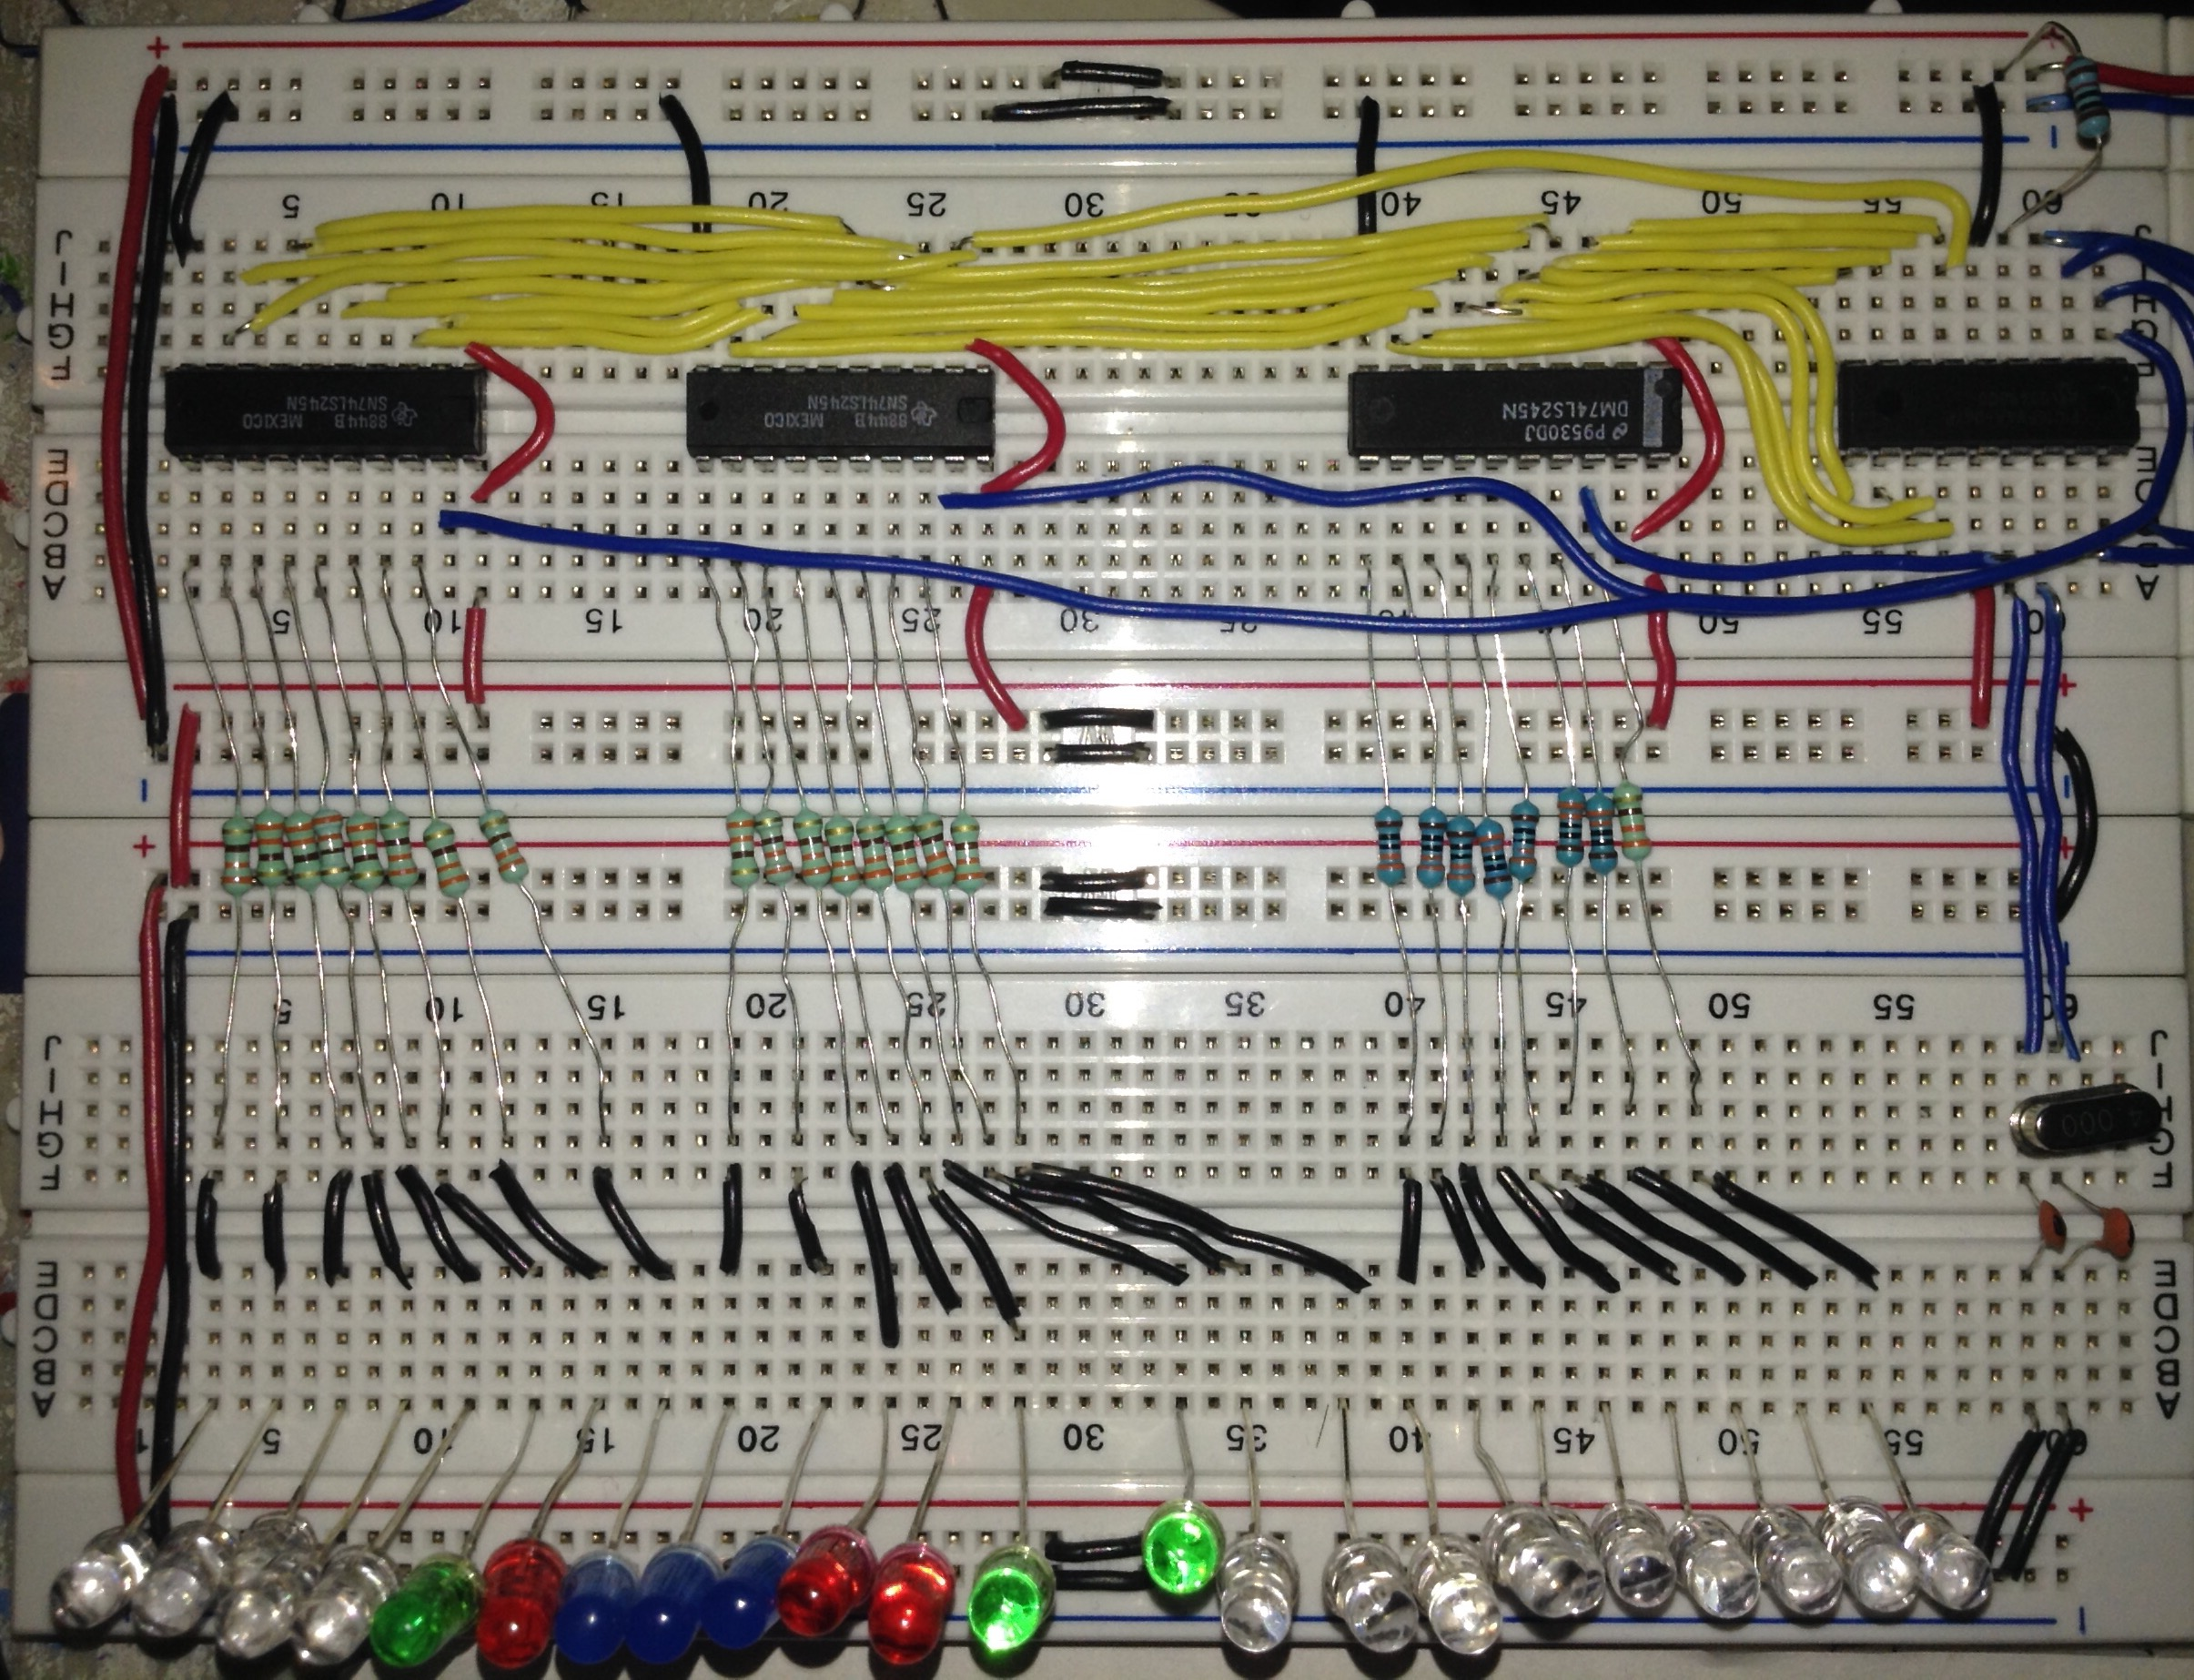
\includegraphics[width=0.45\textwidth]{FullSizeRender3.jpg}
  \caption{Circuito.}
  \label{calentrada}
\end{figure}




 
\section{Resultados }

En las primeras pruebas del circuito no se logro lo esperado, pero despu�s de m�ltiples iteraciones fue posible ver en simulaci�n lo cometido.

\section{Conclusi\'on }
Una secuencia de luces puede llevar a grandes simulaciones si no se sabe con certeza que es lo que hay en los registros, pero al obtener esa informaci�n la realizaci�n de una secuencia se vuelve mas sencillo. 



\end{document}